%
% phi3.tex -- 
%
% (c) 2019 Prof Dr Andreas Müller, Hochschule Rapperswil
%
\documentclass[tikz]{standalone}
\usepackage{amsmath}
\usepackage{times}
\usepackage{txfonts}
\usepackage{pgfplots}
\usepackage{csvsimple}
\usetikzlibrary{arrows,intersections,math}
\begin{document}
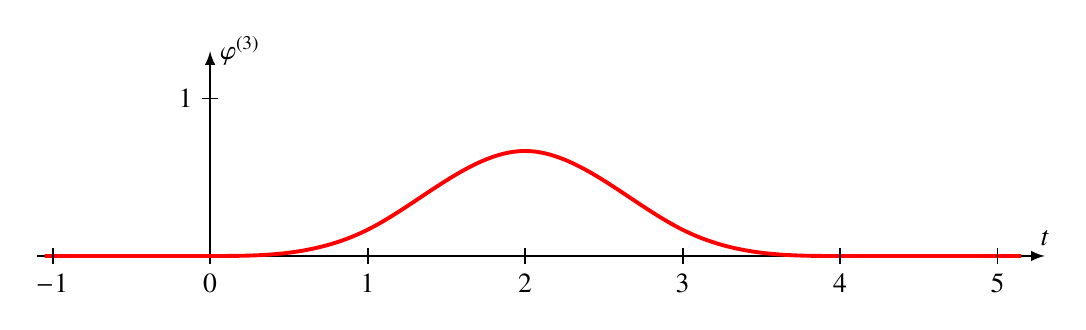
\begin{tikzpicture}[>=latex,scale=2]

\draw[->,line width=0.7pt] (-1.1,0)--(5.3,0)
	coordinate[label={$t$}];
\draw[->,line width=0.7pt] (0,-0.05)--(0,1.3)
	coordinate[label={right:$\varphi^{(3)}$}];

\draw[line width=1.4pt,color=red]
	(-1.05,0)
	--
	plot[domain=0:1,samples=100] ({\x},{\x*\x*\x/6})
	--
	plot[domain=-1:0,samples=100] ({2+\x},{-0.5*\x*\x*\x-\x*\x+2/3})
	--
	plot[domain=0:1,samples=100] ({2+\x},{0.5*\x*\x*\x-\x*\x+2/3})
	--
	plot[domain=3:4,samples=100] ({\x},{-(\x-4)*(\x-4)*(\x-4)/6})
	--
	(5.15,0);

\draw[line width=0.7pt] (-1,-0.05)--(-1,0.05);
\draw[line width=0.7pt] (1,-0.05)--(1,0.05);
\draw[line width=0.7pt] (2,-0.05)--(2,0.05);
\draw[line width=0.7pt] (3,-0.05)--(3,0.05);
\draw[line width=0.7pt] (4,-0.05)--(4,0.05);
\draw[line width=0.7pt] (5,-0.05)--(5,0.05);

\draw[line width=0.7pt] (-0.05,1)--(0.05,1);

\node at (-1,-0.05) [below] {$-1$};
\node at (1,-0.05) [below] {$1$};
\node at (2,-0.05) [below] {$2$};
\node at (3,-0.05) [below] {$3$};
\node at (4,-0.05) [below] {$4$};
\node at (5,-0.05) [below] {$5$};
\node at (0,-0.05) [below] {$0$};

\node at (-0.05,1) [left] {$1$};

\end{tikzpicture}
\end{document}

